\documentclass[10pt,letterpaper]{article}

\usepackage[margin=.5in]{geometry}
%\usepackage{xfrac}
\usepackage{polynom}
\usepackage{tikz}
\usepackage{amsmath}

\usetikzlibrary{calc}
\newcommand{\tikzmark}[1]{\tikz[overlay,remember picture] \node (#1) {};}

\begin{document}
%\everymath{\scriptscriptstyle}
\parindent=0pt
\abovedisplayshortskip=0pt
\belowdisplayshortskip=0pt
\abovedisplayskip=0pt
\belowdisplayskip=0pt
\fbox{ \begin{minipage}{140pt}
\centering All Students Take Calculus

I--All pos. II--sin III--tan IV--cos
\end{minipage}}
\fbox{ \begin{minipage}{96pt}
\centering Law of Cosines
\[
a^2=b^2+c^2-2bc\cdot\cos A
\]
\end{minipage}}
\fbox{\begin{minipage}{117pt}
\centering Difference of Cubes
\[
a^3\pm b^3=(a\pm b)(a^2\mp ab+b^2)
\]
\end{minipage}}
\fbox{ \begin{minipage}{31pt}
\centering Arc Length
\[
s=r\theta
\]
\end{minipage}}

\fbox{ \begin{minipage}{124pt}
\centering Heron's Formula
\[
A=\sqrt{s(s-a)(s-b)(s-c)}
\]
\end{minipage}}
\fbox{ \begin{minipage}{67pt}
\centering Change of Base
\[
\log_bm=\frac{\log m}{\log b}
\]
\end{minipage}}
\fbox{ \begin{minipage}{123pt}
\centering Choose Formula
\[
C(x,y)= {\binom{x}{y}}=\frac{x!}{y!(x-y)!}
\]
\end{minipage}}
\fbox{ \begin{minipage}{100pt}
\centering Law of Sines
\[
\frac{\sin A}{a} = \frac{\sin B}{b} = \frac{\sin C}{c}
\]
\end{minipage}}

\fbox{ \begin{minipage}{84pt}
\centering Degrees to Radians
\[
\frac{A\cdot\pi}{180}=\theta
\]
\end{minipage}}
\fbox{ \begin{minipage}{52pt}
\centering Sector Area
\[
A=\frac12r^2\theta
\]
\end{minipage}}
\fbox{\begin{minipage}{79pt}
\centering Area of $\Delta$
\[
Area = ab\cdot \frac12 \sin C
\]
\end{minipage}}
\fbox{ \begin{minipage}{140pt}
\[
(\log_ab)(\log_cd)=(\log_ad)(\log_cb)
\]
\end{minipage}}

\fbox{ \begin{minipage}{7.36in}
\centering Trig Identities
    
\fbox{\(  \sin^2+\cos^2=1 \)}
\fbox{\(  \tan^2 + 1 = \sec^2 \)}
\fbox{\(  1+\cot^2=\csc^2 \)}
\fbox{\(  2\sin u \cos u=\sin(2u) \)}
\fbox{\(  \cos^2u-\sin^2u=\cos(2u) \)}
\fbox{\(  \frac{2\tan u}{1-\tan^2u}=\tan(2u) \)}
\fbox{\(  \sin u\cos v\pm\cos u\sin v=\sin(u\pm v) \)}
\fbox{\(  \cos u\cos v\mp\sin u\sin v=\cos(u\pm v) \)}
\fbox{\(  \frac{\tan u\pm\tan v}{1\mp\tan u\tan v}=\tan(u\pm v) \)}
\fbox{\(  \cot = \frac1{\tan} \)}
\fbox{\(  \csc = \frac1{\sin} \)}
\fbox{\(  \sec = \frac1{\cos} \)}
\fbox{\(  \sin \left(\frac\pi 2-u\right)=\cos u \)}
\fbox{\(  \tan \left(\frac\pi 2-u\right)=\cot u \)}
\fbox{\(  \sec \left(\frac\pi 2-u\right)=\csc u \)}
\fbox{\(  \cos \left(\frac\pi 2-u\right)=\sin u \)}
\fbox{\(  \cot \left(\frac\pi 2-u\right)=\tan u \)}
\fbox{\(  \csc \left(\frac\pi 2-u\right)=\sec u \)}
\fbox{\(  \frac{1-\cos 2x}{2}=\sin^2x \)}
\fbox{\(  \frac{1+\cos 2x}{2}=\cos^2x \)}
\fbox{\(  \frac{1-\cos 2x}{1+\cos 2x}=\tan^2x \)}
\fbox{\(  \pm\sqrt{\frac{1-\cos u}{2}}=\sin \frac u2 \)}
\fbox{\(  \pm\sqrt{\frac{1+\cos u}{2}}=\cos \frac u2 \)}
\fbox{\(  \frac{1-\cos u}{\sin u}=\frac{\sin u}{1+\cos u}=\tan\frac u2 \)}
\fbox{\(  2\sin\frac{x\pm y}{2}\cos\frac{x\mp y}{2}=\sin x\pm\sin y \)}
\fbox{\(  2\cos\frac{x+y}{2}\cos\frac{x-y}{2}=\cos x+\cos y \)}
\fbox{\(  -2\sin\frac{x+y}{2}\sin\frac{x-y}{2}=\cos x-\cos y \)}
\fbox{\(  \sin u\cos v=\frac12[\sin(u+v)+\sin(u-v)] \)}
\fbox{\(  \cos u\sin v=\frac12[\sin(u+v)-\sin(u-v)] \)}
\fbox{\(  \cos u\cos v=\frac12[\cos(u+v)+\cos(u-v)] \)}
\fbox{\(  \sin u\sin v=\frac12[\cos(u+v)-\cos(u-v)] \)}
\end{minipage}}
\newpage
\fbox{\begin{minipage}{266pt}
\centering Algebra of Functions

\raggedright Let $f$ and $g$ be functions with domains $A$ and $B$.
\[
\begin{array}{cl}
(f+g)(x)=f(x)+g(x) & \textrm{Domain~} A \cap B  \\
(f-g)(x)=f(x)-g(x) & \textrm{Domain~} A \cap B \\
(fg)(x)=f(x)g(x) & \textrm{Domain~} A \cap B \\
\left(\frac{f}{g}\right)(x)=\frac{f(x)}{g(x)} & \textrm{Domain~} \{x \in A \cap B \mid g(x) \neq 0\} \\
(f \circ g)(x)=f(g(x)) & \textrm{Domain~} \{x \in B \mid g(x) \in A\}
\end{array}
\]
\end{minipage}}
\fbox{\begin{minipage}{133pt}
\centering Polynomial Synthetic Division
\[
(x^3+x^2-1) \div (x+2)
\]
\polyset{showbase=top}
\hspace{-7pt}\polyhornerscheme[x=-2,stage=8]{x^3+x^2-1}
\end{minipage}}
\fbox{\begin{minipage}{118pt}
\centering Polynomial Long Division
\polylongdiv[stage=8]{x^3+x^2-1}{x+2}
\end{minipage}}

\fbox{\begin{minipage}{140pt}
\centering Rational Roots Theorem
\[
2x^3+2x^2-3x-6
\] 
\hspace{15pt}$\pm1, \pm2$ \hfill $\pm1, \pm2, \pm3, \pm6$

Possible rational roots:

$\pm1, \pm\frac{1}{2}, \pm2, \pm3, \pm\frac{3}{2}, \pm6$
\end{minipage}}
\fbox{\begin{minipage}{140pt}
\centering Decartes' Rule of Signs

\raggedright Count num. of sign changes
\[
  P(x)=3x^6+4x^5+\tikzmark{a}3x^3-\tikzmark{b}x-3
  \begin{tikzpicture}[overlay,remember picture,out=315,in=225,distance=0.4cm]
    \draw[-latex] (a) to (b);
  \end{tikzpicture}
\]
1 positive real root
\[
  P(-x)=\tikzmark{a}3x^6-\tikzmark{b}4x^5-\tikzmark{c}3x^3+\tikzmark{d}x-\tikzmark{e}3
  \begin{tikzpicture}[overlay,remember picture,out=315,in=225,distance=0.4cm]
    \draw[-latex] (a) to (b);
    \draw[-latex] (c) to (d);
    \draw[-latex,out=290,in=250] (d) to (e);
  \end{tikzpicture}
\vspace*{5pt}
\]
1 or 3 negative real roots
\end{minipage}}
\fbox{\begin{minipage}{140pt}
\centering Logarithm Formulas
\begin{align*}
\log(m\cdot n) &= \log m + \log n \\
\log\left(\frac{m}{n}\right) &= \log m - \log n \\
\log(m^n) &= n \cdot \log m \\
\log_bb^x &= x =b^{\log_bx} 
\end{align*}
\end{minipage}}
\fbox{\begin{minipage}{67pt}
\centering Other trig stuff
\begin{align*}
\cot &= \frac1{\tan} \\
\csc &= \frac1{\sin} \\
\sec &= \frac1{\cos}
\end{align*}
\end{minipage}}

\fbox{\begin{minipage}{216pt}
\centering Horizontal Asymptotes
\begin{align*}
y&=\frac{2x^2-4x+5}{x^2-2x+1} &&\, \textrm{Original Equation}\\
 &=\frac{2x^2}{x^2} &&\, x \to \infty, \textrm{other terms $\to$ tiny}\\
 &=2 &&\, \textrm{Cancel, horizontal asymptote}
\end{align*}
\end{minipage}}
\fbox{\begin{minipage}{212pt}
\centering Slant Asymptotes
\begin{align*}
y&=\frac{x^2-4x-5}{x-3} &&\, \textrm{Original Equation}\\
 &=x-1-\frac{8}{x-3} &&\, \textrm{Divide}\\
 &=x-1 &&\, x\to\infty, \textrm{other terms $\to$ tiny}
\end{align*}
\end{minipage}}

\fbox{\begin{minipage}{181pt}
\centering Vertical Asymptotes
\begin{align*}
y&=\frac{2x^2-4x+5}{x^2-2x+1} &&\, \textrm{Original Equation}\\
 &=\frac{2x^2-4+5}{(2x-1)(x+2)} &&\, \textrm{Factor demoniator}\\
x&=\frac12 \textrm{~or~} x=-2 &&\, \textrm{Impossible}
\end{align*}
\end{minipage}}
\fbox{\begin{minipage}{152pt}
\centering End Behavior

\begin{minipage}{40pt}
\[
y=x^n
\]
$n$ is even\vspace{5pt}
\[
y=x^n
\]
$n$ is odd
\end{minipage}
\begin{minipage}{30pt}
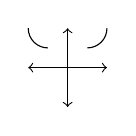
\begin{tikzpicture}
  \draw[<->] (-.5,0) -- (.5,0);
  \draw[<->] (0,-.5) -- (0,.5);
  \draw[in=270,out=0] (.25,.25) to (.5,.5);
  \draw[in=270,out=180] (-.25,.25) to (-.5,.5);
\end{tikzpicture}
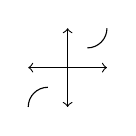
\begin{tikzpicture}
  \draw[<->] (-.5,0) -- (.5,0);
  \draw[<->] (0,-.5) -- (0,.5);
  \draw[in=270,out=0] (.25,.25) to (.5,.5);
  \draw[in=90,out=180] (-.25,-.25) to (-.5,-.5);
\end{tikzpicture}
\end{minipage}~
\begin{minipage}{40pt}
\[
y=-x^n
\]
$n$ is even\vspace{5pt}
\[
y=-x^n
\]
$n$ is odd
\end{minipage}
\begin{minipage}{30pt}
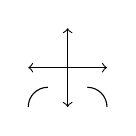
\begin{tikzpicture}
  \draw[<->] (-.5,0) -- (.5,0);
  \draw[<->] (0,-.5) -- (0,.5);
  \draw[in=90,out=0] (.25,-.25) to (.5,-.5);
  \draw[in=90,out=180] (-.25,-.25) to (-.5,-.5);
\end{tikzpicture}
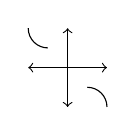
\begin{tikzpicture}
  \draw[<->] (-.5,0) -- (.5,0);
  \draw[<->] (0,-.5) -- (0,.5);
  \draw[in=90,out=0] (.25,-.25) to (.5,-.5);
  \draw[in=270,out=180] (-.25,.25) to (-.5,.5);
\end{tikzpicture}
\end{minipage}
\end{minipage}}

\fbox{\begin{minipage}{207pt}
\centering $y=\sin x$ in red; $y=\cos x$ in blue
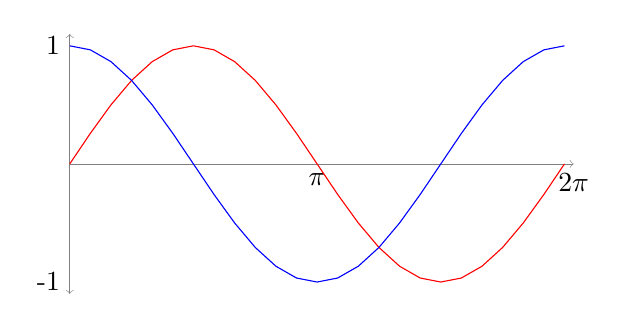
\begin{tikzpicture}[yscale=1.5]
\draw [help lines, ->] (0,0) -- (6.4,0);
\node [below] at (6.4,0) {$2\pi$};
\node [below] at (pi,0) {$\pi$};
\node [left] at (0,1) {1};
\node [left] at (0,-1) {-1};
\draw [help lines, <->] (0,-1.1) -- (0,1.1);
\draw [red,domain=0:2*pi] plot (\x, {sin(\x r)});
\draw [blue, domain=0:2*pi] plot (\x, {cos(\x r)});

\end{tikzpicture}
\end{minipage}}
\fbox{ \begin{minipage}{110pt}
\centering sin/cos Graph Properties

\raggedright If in form:
\[
y=a\sin k(x-b)
\]
amplitude  $|a|$, period  $2\pi/k$, phase shift $b$
\end{minipage}}
\end{document}
